\chapter{Using waves to represent information}

%\section{Information, numbers and modulation}

In the study of communication, modulation is the subject devoted to how information being represented by physical characteristics of waves. The wealth of knowledge can be applied to not only quantum communication protocols but also to quantum computing.

Radio broadcasts first used radio waves' amplitudes to represent the volume of one's voice. This is the so called amplitude modulation (AM). Later, frequency modulation (FM) was found less prone to noise in the airways. That is why we now have both AM and FM on the panels of our radios. Modern communication also use phase modulation (PM) and quadrature amplitude modulation (QAM) -- the latter is a combination of phase and amplitude modulation.

Quantum devices, working with the smallest quanta of waves, use many of modulation schemes invented for communication with their own twist. Understanding how modulation works in quantum devices is the critical link for engineers to understand quantum technologies.

\subsection{Phase modulation}
Phase modulation uses a wave's phase to represent information. By varying the phase while keep the wave's frequency and amplitude constant, the real numbers in the [0, 2$\pi$) domain can be represented. In communication textbooks, we use the points in constellation diagrams to depict the amplitudes and phases of waves -- 
the distance of a point to the origin is the amplitude of the wave, and the angle to the x-axis $\phi$ is the phase. 
So, the numbers that PM can represent fall all onto a circle in a constellation diagram as in Fig. \ref{PM}. Communication textbooks refer the numbers symbols. The range or set of the symbol is called the symbol constellation or symbol set. For example, the symbol constellation of PM in set notation is $phi in [0, 2\pi)$.
(Constellation diagrams are most useful for understanding QAMs, in which both amplitudes and phases are used to represent information.)

%\node [constellation_cir] at (0,0) {};
\begin{figure}[ht]
\begin{tikzpicture}
    \draw[->] (-3.5,0) -- (3.5, 0);
    \draw[->] (0,-3.5) -- (0,3.5);
    \draw[dotted, red] (0,0) circle(3cm);
    \draw[red, fill] (30:3) circle(0.05cm);
    \draw[dashed] (1,0) arc (0:30:1) node[right, pos=0.6]{$\varphi$ - phase};
    \draw[dashed] (30:0.1) -- (30:2.9) node[pos=0.5, rotate = 30, above] {amplitude};
\end{tikzpicture}
\caption{Constellation diagram of phase modulation}
\label{PM}
\end{figure}

\subsection{Digital modulation}
In theory, we can measure a wave's amplitude, frequency and phase precisely and use them to represent real numbers. In really, communication channels and information processing devices have noises and errors. We are best to have the systems working with only integer numbers. Using integer numbers to represent information is what we call digital technology. Further, using binary integers instead of decimals makes computer and communication components much simpler. And nowadays digital technology is almost the synonym of binary technology. Technologies of dealing with real numbers are called analog technologies.

All computers use digital technology if we ignore the history of the slide rule calculators. Even abacuses are digital calculators. Communication systems are slow to convert to digital technology. For a long time, communication was mostly about voice communication -- radio broadcast and telephones -- and used analog technologies. For digital information, modulations such as AM, FM and PM often carry different names, e.g. amplitude-shift keying (ASK), frequency-shift keying (FSK) and phase-shift keying respectively (PSK).

\subsection{Channel capacity and Hartley's law}
Channel capacity measures the maximum possible bits per second of a communication channel. When modulation is the only limitation, Hartley's law gives the channel capacity to be
\begin{equation}
    C = f ln M
\end{equation}
where $f$ being the channel used rate and $M$ being the number of modulation points.

\section{Quadrature phase-shift keying}
Quadrature phase-shift keying (QPSK) uses carrier waves of phases 90 degree apart, for example of phases 0, 90, 180, 270 degrees, to represent 2-bit numbers -- 0, 1, 10, or 11 in binary. A wave with 90 degree phase is called the quadrature wave while the wave with zero phase is called the in-phase wave.
(The significance of using waves with phases 90 degree apart is that every two waves of such phase difference are orthogonal to each other. Therefore, when receiving a wave of phase 180 degree representing "10", which has zero measurement overlap with waves of 90 or 270 degree phases, and has zero probability of being demodulated as "1" or "11".
waves are orthogonal to each other. Measurement of orthogonal waves is least prone to noise or errors 
because they have zero overlap.)

The constellation diagram is shown in the diagram in \ref{QPSK}.

\begin{figure}[ht]
\begin{tikzpicture}
    \draw[->] (-3.5,0) -- (3.5, 0);
    \draw[->] (0,-3.5) -- (0,3.5);
    \draw[dotted, red] (0,0) circle(3cm);
    \draw[red, fill] (3,0) circle(0.05cm) node[below right] {0};
    \draw[red, fill] (0,3) circle(0.05cm) node[above right] {1};
    \draw[red, fill] (-3,0) circle(0.05cm) node[above left] {10};
    \draw[red, fill] (0,-3) circle(0.05cm) node[below left] {11};
\end{tikzpicture}
%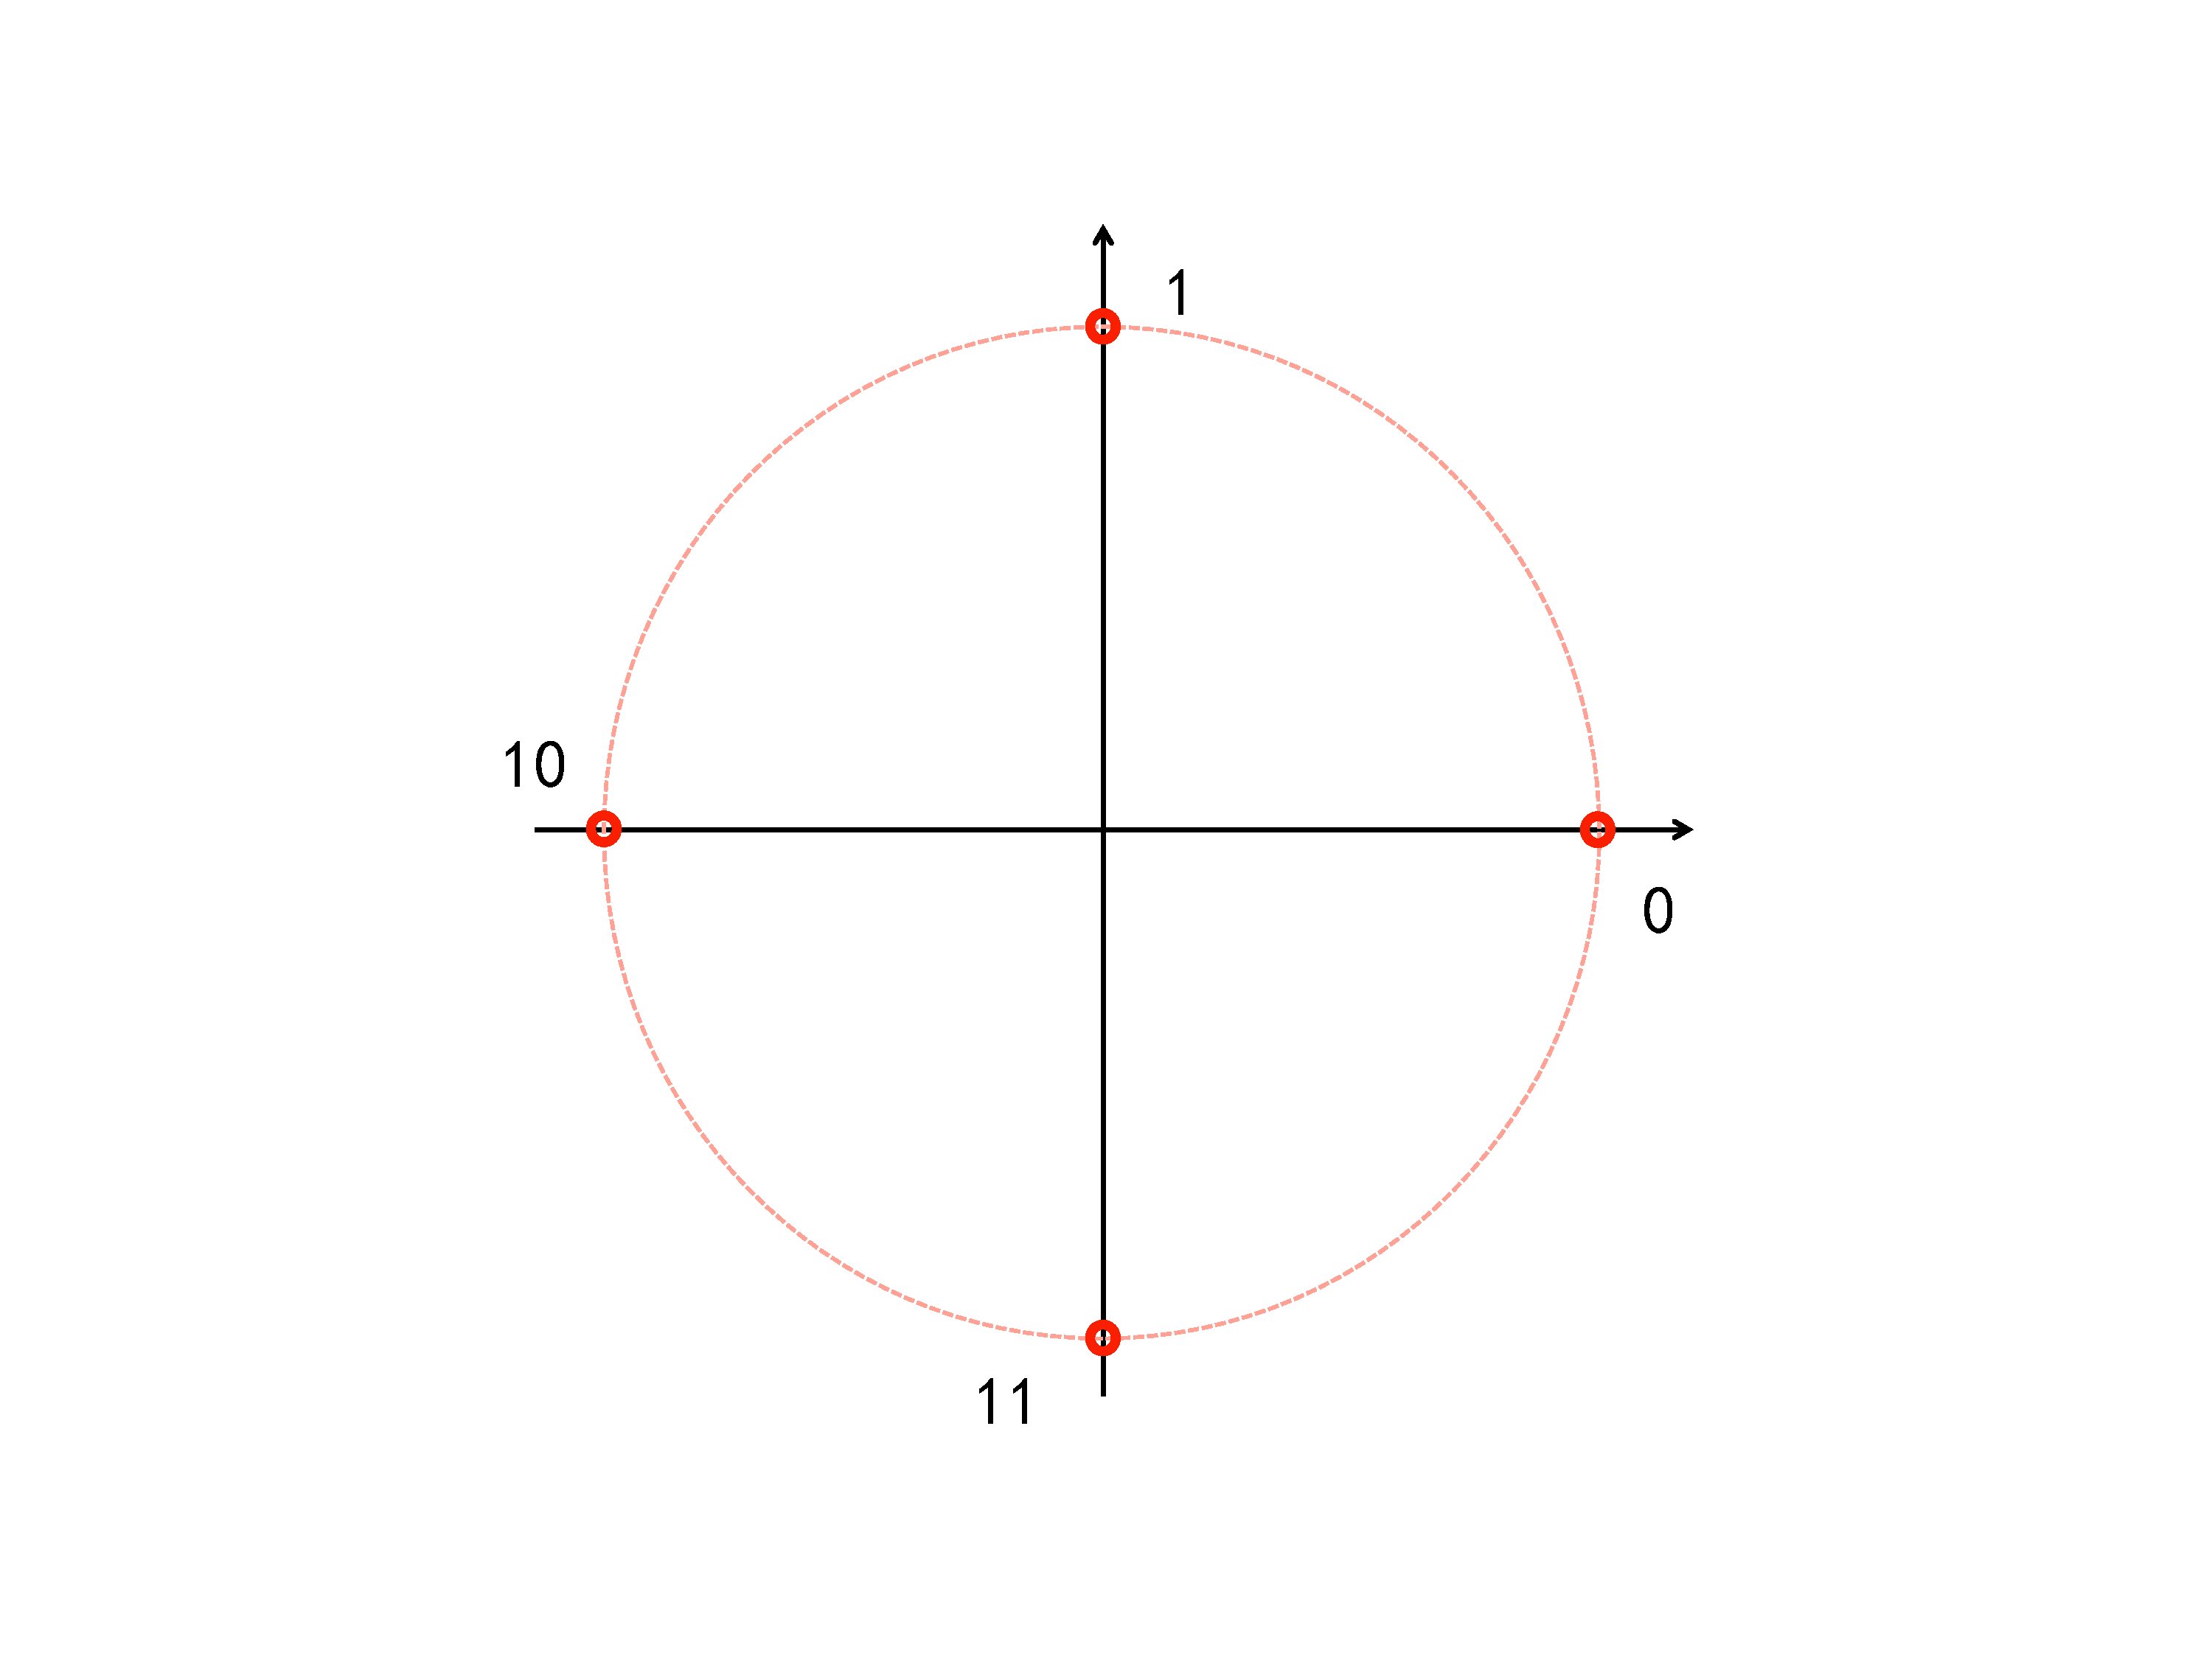
\includegraphics[width=6cm]{pic/4qpsk.pdf}
\caption{QPSK constellation diagram}
\label{QPSK}
\end{figure}

\subsection{Symmetric QPSK}
For simpler modulator circuitry, the QPSK modulation scheme shown in the constellation diagram Fig. \ref{sQPSK} is more widely used in practice.
\begin{figure}[hb]
\begin{tikzpicture}
    \draw[->] (-3.5,0) -- (3.5, 0);
    \draw[->] (0,-3.5) -- (0,3.5);
    \draw[dashed] (2.5,2.5) -- (0, 0);
    \draw[dotted, red] (0,0) circle(3cm);
    \draw[red, fill] (2.12,2.12) circle(0.05cm) node[right] {11};
    \draw[red, fill] (-2.12,2.12) circle(0.05cm) node[above] {01};
    \draw[red, fill] (2.12,-2.12) circle(0.05cm) node[below] {10};
    \draw[red, fill] (-2.12,-2.12) circle(0.05cm) node[left] {00};
    \draw[dashed] (1,0) arc (0:45:1) node[right, pos=0.6]{$\varphi=45\circ$};
\end{tikzpicture}
\caption{Practical QPSK constellation diagram}
\label{sQPSK}
\end{figure}

\subsection{Modulator, demodulator and superposition}
A practical QPSK modulator circuit is shown in Fig. \ref{modulator}. It uses one carrier wave generator and splits the carrier wave into two waves of equal amplitudes. One of the half becomes the quadrature wave after a 90-degree phase shifter while the other half remains as the in-phase wave. modified scheme: in every time slot, 2 bits are fed into the modulator. Each bit is used to modulate a base carrier wave's phase. The two base carrier waves are orthogonal, one of zero phase and the other of 90-degree in phase. If the input to a carrier is "0", its phase is shifted another 180 degrees. The combined or summed up wave of the two carriers is the output of the modulator going into the communication channel. The constellation diagram this scheme is shown in Fig. \ref{QPSK}.

We see that one wave from the source can be divided up into two waves, which can then be combined into one after modulation. In fact, all waves can be combined into one and may be regarded as one wave if they are coherent with each other -- their phases are correlated. Combination, mixing or composing several waves into one is the same concept as superposition in quantum physics although the latter refers to combination, mixing or composition of waves with equal number of quanta.

\begin{figure}[ht]
\begin{tikzpicture}
    \path %(-5,0) node[anchor=east] (start) {Wave} 
    (-3.5,-0.8) node[circle, draw=black] (lo) {$\sim$}
    (-3.5,0.8) node[Gate] (p90) {$90^\circ$}
    (0,2) node[Gate, text width=30] (tm) {$0/180^\circ$}
    (0,-2) node[Gate, text width=30] (bm) {$0/180^\circ$}
    (2,0) node[circle, draw=black] (add) {+}
     (3,0) node[anchor=west] (output) {wave output};
    \draw (lo.east) node[anchor=west] {carrier wave generator};
    \draw (p90.east) node[anchor=west] {phase shifter};
    \draw (tm.north east) node[anchor=west] {variable phase shifter};
    \draw (bm.south east) node[anchor=west] {variable phase shifter};
    \draw (lo) -- (p90) |- (tm) -| (add);
    \draw (lo) |- (bm) -| (add);
    \draw (add) -- (output);
    \path (-2,3) node[anchor=east] (even) {data input - even bits}
    (-2,-3) node [anchor=east] (odd) {data input - odd bits};
    \draw[double] (even) -| (tm);
    \draw[double] (odd) -| (bm);
\end{tikzpicture}
\caption{QPSK modulator circuit}
\label{modulator}
\end{figure}

Figure \ref{deodulator} shows a demomulator circuit, which reverses the modulation: the received signal wave is divided into two waves to be resonated with two local oscillators, which are from the same local source but are orthogonal to each other. The the proportions of the two resonations determine the phase angle of the incoming wave. Bit numbers are output according to the phase angle.

\begin{figure}[ht]
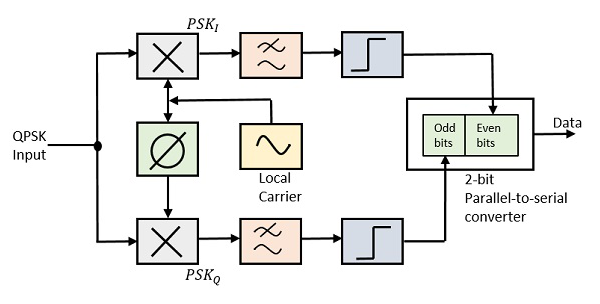
\includegraphics[width=6cm]{pic/qpsk_demodulator.jpg}
\caption{QPSK demodulator circuit}
\label{deodulator}
\end{figure}

\section{Quadrature amplitude modulation}
Quadrature amplitude modulation (QAM) is a combination of amplitude modulation and phase modulation. Modern radio communication such as Wi-Fi and mobile communications all use the digital forms of QAMs.
\begin{figure}[ht]
\begin{tikzpicture}
    \draw[->] (-3.5,0) -- (3.5, 0);
    \draw[->] (0,-3.5) -- (0,3.5);
    \draw[dotted, red] (0,0) circle(3cm);
    \draw[red, fill] (2,0) circle(0.05cm) node[below] {0};
    \draw[red, fill] (0,2) circle(0.05cm) node[right] {1};
    \draw[red, fill] (-2,0) circle(0.05cm) node[above] {10};
    \draw[red, fill] (0,-2) circle(0.05cm) node[left] {11};
    \draw[red, fill] (3,0) circle(0.05cm) node[below right] {100};
    \draw[red, fill] (0,3) circle(0.05cm) node[above right] {101};
    \draw[red, fill] (-3,0) circle(0.05cm) node[above left] {110};
    \draw[red, fill] (0,-3) circle(0.05cm) node[below left] {111};
\end{tikzpicture}
\begin{tikzpicture}
    \draw[->] (-3.5,0) -- (3.5, 0);
    \draw[->] (0,-3.5) -- (0,3.5);
    \draw[dashed] (2.5,2.5) -- (-2.5,-2.5);
    \draw[dashed] (-2.5,2.5) -- (2.5,-2.5);
    \draw[dotted, red] (0,0) circle(3cm);
    \draw[red, fill] (45:2) circle(0.05cm) node[above left] {11};
    \draw[red, fill] (135:2) circle(0.05cm) node[above right] {01};
    \draw[red, fill] (225:2) circle(0.05cm) node[above left] {00};
    \draw[red, fill] (-45:2) circle(0.05cm) node[above right] {10};
    \draw[red, fill] (45:3) circle(0.05cm) node[right] {111};
    \draw[red, fill] (135:3) circle(0.05cm) node[left] {101};
    \draw[red, fill] (225:3) circle(0.05cm) node[left] {100};
    \draw[red, fill] (-45:3) circle(0.05cm) node[right] {110};
\end{tikzpicture}
\caption{Constellation diagrams of two 8QAM systems}
\label{8QAM}
\end{figure}

\section{Polarization modulation}
Polarization modulation is used in optical fiber communication. For example, dual polarization quadrature phase shift keying (DP-QPSK) modulation is a widely used.

\begin{figure}[h]
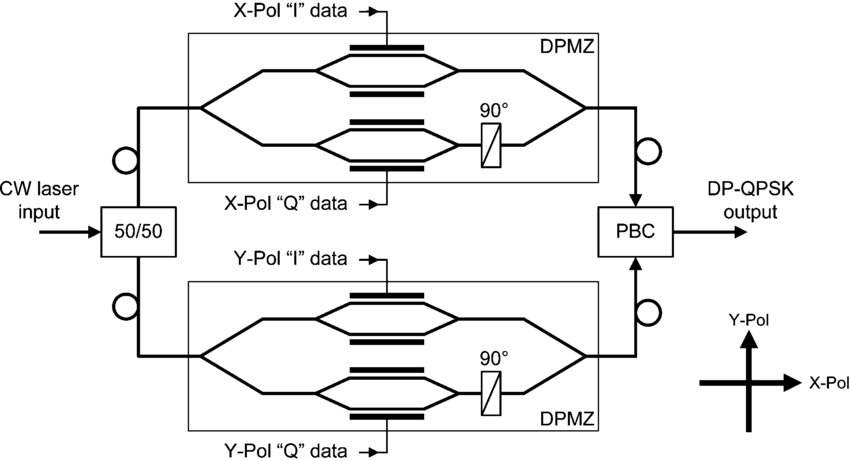
\includegraphics[width=12cm]{pic/DP-QPSK-modulator.png}
\caption{DP-QPSK modulator}
\label{DP-QPSK}
\end{figure}

\chapter{Quantum information}\label{C-qi}
\section{Quantum concepts}
For engineers, only two concepts of quantum physics are needed: 1. all matters are waves even the seemingly size-less electrons and protons are; 2. all waves have their smallest drops, which cannot be divided. Physicists refer the two concepts the partical and wave duality of matters. The first concept tells us that, not limited to radio and optical waves, electrons and protons can also be used to make qubits. However, the implication of the second concept is far more profound and is not explored by traditional communication theory. One implication is that analog amplitude modulation is not possible because amplitude depends on the number of quanta in the wave and can only be use for digital modulation. Second, each qubit can only be measured once.

\subsection{Limitation of measurement}
The final stage of demodulation involves measuring the wave's mass or energy. The result is always a discrete number -- 1, 2, ..., or $n$ -- quanta of mass or energy. The amplitude of the wave is usually proportional to the square root of the mass or energy and takes only discrete values although not exactly 1, 2, ... or $n$.

Measurement always involve energy or mass exchange between the wave and the measurement apparatus. When measuring a photon, for example, its energy is transferred to an electron, and the movement or change in the electron induces an electrical current observable to humans. Lost all the energy to the electron, the photon is "annihilated" -- in physicists' lingo -- and cannot be measured again. The unique feature of quantum information is that we can modulate a qubit device as much information as the cardinal of real numbers but that we can only measure at most once per quantum.

\subsection{Quantum terminology}
By tradition, physicists keep on using the term particle, which may cause the biggest confusion. To most people, particles have the image of point like or of negligible sizes. Physicists believed electrons were point-like in size when JJ Thomson discovered them in 1897. But when Ernest Rutherford discovered atomic nucleus 14 years later, people raised the question: why is the size of an atom much bigger than that of its nucleus? Why wouldn't the tiny negatively charged electrons fall into the positively charged nucleus and be combined into an atom close to the size of the nucleus -- if it were to happen, we would have not seen the world as we have.

Physicists refer the drop-like behavior of electrons and all other matters as the particle behavior. "Quantum" should have been the perfect word in place of particle, but we think "drop" is a better word for non-physicists to understand.

Beside particle, physicists use the term "state" to refer the wave of one drop. It is the same concept as "mode" in the context of optical communication and photonics. It is used to describe a wave when the absolute amplitude value is known or unimportant. But the term carries many different meanings to engineers. We will believe it's wise to use the term "wave" in place of state. By tradition, physicists use the so-called Dirac "bra-ket" notation to label quantum states. In the ket notation, the base carrier waves are noted as $\keta{0}$ and $\keta{1}$.

When talking about electrons being waves, people are often puzzled and ask what is vibrating in an electron wave. Physicists are puzzled too and have been debating the possibilities without conclusion. Engineers don't have to interject into the debate and need only know that an electron wave qubit has frequency, phase and polarization for modulating.

\section{Qubit modulation}
\subsection{Requirements on modulation}
We have two conflicting requirements when considering how to modulate a qubit:
\begin{itemize}
    \item For parallel computing/exploration, the modulation points should be as many as possible.
    \item For output, the measurable modulation points are limited to the "0" and "1" points.
\end{itemize}

The first requirement is easy to understand, and phase modulation, with modulation points $\phi \in [0, 2\pi)$, meets the requirement. The second requirement is due to that fact that one qubit has only one quantum of wave, which resonates with only one of the local oscillators in the demodulator as shown in Fig. \ref{deodulator} and never both.

As described in the Appendix on qubit devices, all devices add a second modulation such as polarization, frequency, mode modulation or the like to meet the second requirement. In this book, we refer these secondary modulations a generic term, $\theta$ modulation, because all of them can be characterized by an angle value $\theta \in (-\pi/2, \pi/2]$ as discussed in the appendix on qubit devices.

\subsection{Measurable modulation points}
\subsubsection{Quadrature amplitude modulation}
Since a wave is in quanta, 1, 2, 3, ..., or n quanta, its amplitude is discrete too although not in increment of 1, 2, 3, ..., or n. Adding amplitude modulation is by adding more qubits and can be used only for digital modulation. Amplitude modulation is always used to add code points for digital modulation and cannot be used for parallel computing.

\subsection{Analog modulation}
Analog modulation can only be used at input or in processing. For communication, each qubit actually has two channels -- $\theta$ and $\varphi$. And their channel capacities per qubit duty cycle are $\theta \in (-\pi/2, \pi/2] and \varphi \in [0, \pi)$. For computing, that is the capacities are the amount of information a qubit can store.

\subsection{Demodulation and quantum measurement}
When a cellphone receives a radio wave, the demodulator can divide the wave into many portions to measure the amplitudes and phases. But with a qubit, although we can adopt any of the modulation technique and put information in any of the data points $(\theta, \varphi)$, we cannot divide one quantum of wave for multiple measurement.

Similar to a demodulator of QPSK. a demodulator of a qubit expose the quantum of wave to two electronic resonators orthogonal to each other.  If we know the qubit is modulated by BQSK, detecting the qubit in the $\keta{0}$ wave means the qubit's phase $\theta = 0$. Further, the absence of detecting signal in the $\keta{1}$ wave also suggests $\theta = 0$ too. But if the qubit is originally modulated in any other way, we have no way of measuring the knowing the information that the qubit represents. the probability of one resonator responds to the wave depends on how much the resontor overlaps with the wave in space and time.

In contrast to conventional communication and computing systems, information entered into a quibit may be lost at demodulation or measurement. That is the unique feature of quantum information.

\subsection{Wave characteristics for qubit modulation}
\begin{table}[]
\caption{Wave characteristics for qubit modulation}
\label{modulation-characteristics}
\begin{tabular}{lll}
Wave parameters &Represented numbers &Qubit design   \\
Amplitude & Number of qubits 1, 2, ... & all qubits \\
Phase & $\varphi \in (-\pi /2, \pi /2] $& all qubits \\
Frequency & $\theta \in (-\pi /2, \pi /2]$ & SC-IBM, Google; trapped ion - IonQ \\
Mode & $\theta \in (-\pi /2, \pi /2]$ & Xanadu, PsiQuantum \\
Polarization & $\theta \in (-\pi /2, \pi /2]$ & USTC \\
Spin & $\theta \in (-\pi /2, \pi /2]$ & 
\end{tabular}
\end{table}

\section{Mathematical notation of qubit modulation}
From communication theory perspective, a qubit is best described by the parameter pair $(\theta, \varphi)$. But other notations developed by physicists may be easier to use when working on problems involving more than one qubit. 
\subsection{Ket notation}
Summing up the base carriers, the superposition wave can be noted as $\keta{s} = cos{\theta} \keta{0} + e^{i \varphi} sin{\theta} \keta{1}$ or simply $\keta{s} = a \keta{0} + b \keta{1}$. Here, the $+$ sign means wave addition but has no mathematical meaning. And $a$ and $b$ are complex numbers and reflect the amplitude and phase contributions to the superposition. Even with the constraint $|a|^2+ |b|^2$, this notation includes waves $e^{i\lambda} (cos{\theta} \keta{0} + e^{i \varphi} sin{\theta})$ which are the same except their global phase $\lambda$.

\subsection{Vector notation}
For mathematicians and computer scientists, the physical meaning of wave addition can be ignored, and the vector notation $
\begin{pmatrix}
    a \\
    b
\end{pmatrix}$ is best for derivation and calculation.

But not all of the 4 real numbers the two complex numbers can be used independently for modulation. First, the amplitude of the wave is one to be sure that the qubit contains only one quantum $|a|^2 + |b|^2 = 1$.
\begin{equation}
    \begin{pmatrix}
    cos\theta & -e^{i\lambda} sin\theta \\
    e^{i\varphi} sin\theta & e^{i(\varphi + \lambda)} cos\theta
\end{pmatrix}
\end{equation}
Any operation rotates the data point of a qubit on the Bloch sphere and can be described by the triplet of Euler angles, $\delta \theta, \delta \varphi, \delta \lambda$. The matrix notation is
\begin{equation}
    \begin{pmatrix}
        cos\delta \theta & -e^{i\delta \lambda} sin\delta \theta \\
        e^{i \delta \varphi} sin\delta \theta & e^{i \delta \varphi+ \delta \lambda} cos\theta 
    \end{pmatrix}
\end{equation}

\subsection{Binary numbers}

If we measure waves in any other way than space or time, we find their smallest "drops" -- the particle nature of matter. Quantum physics started a hundred years ago when Einstein first proposed that electromagnetic waves, when measured in their energy, have the smallest drops called photons.

When measuring in electric charge, physicists discovered the smallest drops first and call them electrons before they realized their wave nature.

Measurement is the very thing that the quantum world is different from the classical world. In the quantum world, with an article, you only have one chance to measure it.)

Digital technologies gain precision over analog technologies but lose in the amount of information they can carry. The amount of information that a modulation technique can carry relates to the size or cardinality of the set of numbers that it can represent. With analog PM, the cardinality of the set [0, 2$\pi$) is infinity and is the same as the entire set of real numbers. But the set of integers that a digital modulation represent is finite. And the amount of information that a digital communication channel carries per time slot is finite. To increase the communication speed, the cellphone industry has been trying to squeeze more and more information per time slot by adopting increased data points of QAM modulations -- 4QAM, 8QAM, 16QAM ....
From the above description of the various types of qubits, we see that they all have the pseudo phase $\theta_p$ to characterize the 
orthogonality or overlap among the waves in the polarization, spatial or frequency domains, and can be used represent real numbers in the $\{\theta_p \in [0, \pi/2)\}$ domain. In addition, the relative phase in the time domain of the two base carrier waves in a qubit is another independent variable that can be. Physicists usually use $\theta_q = \theta_p/2 \keta{0}$ and the Bloch sphere as in Fig. \ref{Bloch} to draw an intuitive picture of the entire modulation domain of a qubit $\{\theta_q \in [0, \pi]$ and $\phi \in [0, 2\pi)\}$.

\begin{table}[]
\caption{Parameters and ranges for modulation}
\label{modulation-parameters}
\begin{tabular}{lll}
Parameter &Represented numbers &Note                 \\
Amplitude &Number of qubits $\in \{1, 2, 3, ...\}$   & None \\
Phase & $\varphi \in (-\pi /2, \pi /2] $& Z gate \\
Polarization angle (spatial overlap) & $\theta \in (-\pi /2, \pi /2]$ &X gate
\end{tabular}
\end{table}

\section{Graphical depictions}
\subsection{Quarter sphere diagram}
\begin{figure}[ht]
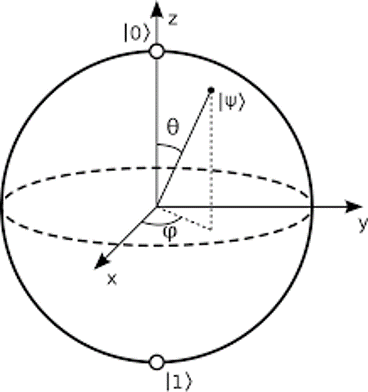
\includegraphics[width=6cm]{pic/blochSphere.png}
\caption{Bloch sphere}
\label{Bloch}
\end{figure}

\begin{figure}[ht]
\tdplotsetmaincoords{0}{0}
\begin{tikzpicture} %[scale=2,tdplot_main_coords]
 \def\rvec{3}
 \def\thetavec{50}
 \def\phivec{40}
 
    %Axes
    \coordinate (O) at (0,0,0);
    \draw[dashed, ->] (0,0,0) -- ++(3.5, 0,0) node[below,right] (x) {x};
    \draw[dashed, ->] (0,-3.5,0) -- ++(0, 7, 0) node[above,right] (y) {y};
    \draw[dashed, ->] (0,0,0) -- ++(0, 0, 3.9) node[below] (z) {$\omega t$};
    \draw[] (0,-3) arc(-90:90:3 and 3);
    \draw[] (0,3) arc (90:270:1.3 and 3);
    \draw[] (-1.2,-1.2) arc (-113:0:3 and 1.35);
    \draw[] (3,0,0) -- ++(0.5, 0, 0);
    \draw[] (0,-3.5,0) -- ++(0, 0.5, 0);
    \draw[] (0,3,0) -- ++(0, 0.5, 0);
    \draw[] (0,0,3) -- ++(0, 0, 0.5);

    % Vector
    \tdplotsetcoord{P}{\rvec}{\thetavec}{\phivec}
    \draw[red,fill] (P) circle(0.05);
    \draw[dashed, red] (O) -- (P) node[circle] (Ptheta) {};
    \draw[dashed, red] (O) -- (Pyz) node[circle] (Pphi) {};
    \draw[dashed, red] (P) -- (Pyz);
    %\draw[dashed, red] (Px) -- (Pxz);

    % angles;
    \draw [shift={(0,0)}, lightgray, fill, fill opacity=0.1] (0,0) -- (P) arc (35:0:1.2) -- cycle;
    \draw [shift={(0,0)}, lightgray, fill, fill opacity=0.1] (0,0) -- (Pyz) arc [start angle=125, delta angle=-12, radius=3.9 ] -- cycle;
    %\draw [shift={(0,0)}, lightgray, fill, fill opacity=0.1] (0,0) -- (Pyz) arc (75:60:1.2) -- cycle;
    \draw( -0.8, 1.6) node[anchor=north west] {$\varphi$};
    \draw( 1.3, 0.8) node[anchor=north west] {$\theta$};
\end{tikzpicture}
\caption{Qubit modulation space}
\label{bloch-alt}
\end{figure}

\subsection{Bloch sphere}
\begin{figure}[ht]
\tdplotsetmaincoords{0}{0}
\begin{tikzpicture} %[scale=2,tdplot_main_coords]
 \def\rvec{3}
 \def\thetavec{70}
 \def\phivec{60}
 
    %Axes
    \coordinate (O) at (0,0,0);
    \draw[->] (0,0,0) -- ++(3.5, 0,0) node[below,right] (y) {y};
    \draw[->] (0,0,0) -- ++(0, 3.5, 0) node[above,right] (z) {z};
    \draw[->] (0,0,0) -- ++(0, 0, 3.5) node[below] (x) {x};
    \draw[] (0,0) circle(3);
    \draw[orange] (-3,0) arc (180:360:3 and 1);
    \draw[dashed, orange] (3,0) arc (0:180:3 and 1);

    % Vector
    \tdplotsetcoord{P}{\rvec}{\thetavec}{\phivec}
    \draw[red,fill] (P) circle(0.05);
    \draw[dashed, red] (O) -- (P) node[circle] (Ptheta) {};
    \draw[dashed, red] (O) -- (Pxz) node[circle] (Pphi) {};
    \draw[dashed, red] (P) -- (Pxz);
    %\draw[dashed, red] (Px) -- (Pxz);

    % angles;
    \draw [shift={(0,0)}, lightgray, fill, fill opacity=0.1] (0,0) -- (65:0.8) arc (65:90:0.8) -- cycle;
    \draw [shift={(0,0)}, lightgray, fill, fill opacity=0.1] (0,0) -- (-135.7:0.6) arc (-135.7:-25:0.6) -- cycle;
    \draw( -0.1, -0.6) node[anchor=north west] {$\varphi$};
    \draw( 0.05, 1.5) node[anchor=north west] {$\theta_B$};
\end{tikzpicture}
\caption{Bloch sphere}
\label{bloch}
\end{figure}

\subsection{Constellation diagrams}
Constellation diagrams are familiar to engineers and are great graphical illustration of modulations involving only phase and amplitude. But quantum devices add $\theta$ modulation.

\section{Mostly used modulation points}\label{Sec-Plus}
\subsection{$\keta{1}$}
$\keta{1}$ is one of the base waves of a qubit. However, quantum computing circuit diagrams usually assume all input waves are $\keta{0}$, and assume a $\keta{1}$ wave being transformed by an X gate from a $\keta{0}$ wave --
$\keta{1} = X \keta{0}$ -- in ket notation. In vector notation, the $X$ gate has a matrix representation
\begin{equation}
    X = \begin{pmatrix}
        0 & 1 \\
        1 & 0
    \end{pmatrix}.
\end{equation}
In circuit notation,
\begin{figure}[ht] \label{X1}
\begin{quantikz}
    \lstick{\ket{0}} & \gate{X} & \qw \rstick{\ket{1}}
\end{quantikz}
\caption{Use X gate to produce $\keta{1}$ wave.}
\end{figure}
The X gate can also be represented as $\bigoplus$. But in this book, we do not use this notation.

We see that an X gate flips the bases $\keta{0}$ and $\keta{1}$ from one to another. 

\subsection{The $\keta{+}$ and $\keta{-}$ waves}
To read out from a qubit, it must be in a binary modulation. Similar to QPSK shown in Fig. \ref{qQPSK}, we can map the modulation points $\theta=0$ and $\pi/2$ to represent "0" and "1" respectively as shown in the constellation diagram Fig. \ref{QPSK} 
\begin{figure}[hp]
\begin{tikzpicture}
    \draw[->] (-3.5,0) -- (3.5, 0);
    \draw[->] (0,-3.5) -- (0,3.5);
    \draw[dashed] (2.5,2.5) -- (0,0);
    \draw[dashed] (0,0) -- (2.5,-2.5);
    \draw[dotted, red] (0,0) circle(3cm);
    \draw[red, fill] (3,0) circle(0.05cm) node[below right] {0};
    \draw[red, fill] (0,3) circle(0.05cm) node[above right] {1};
    \draw[red, fill] (2.12,2.12) circle(0.05cm) node[right] {11};
    \draw[red, fill] (2.12,-2.12) circle(0.05cm) node[below] {10};
    \draw[dashed] (1,0) arc (0:45:1) node[right, pos=0.6]{$\theta=\pi/4$};
\end{tikzpicture}
%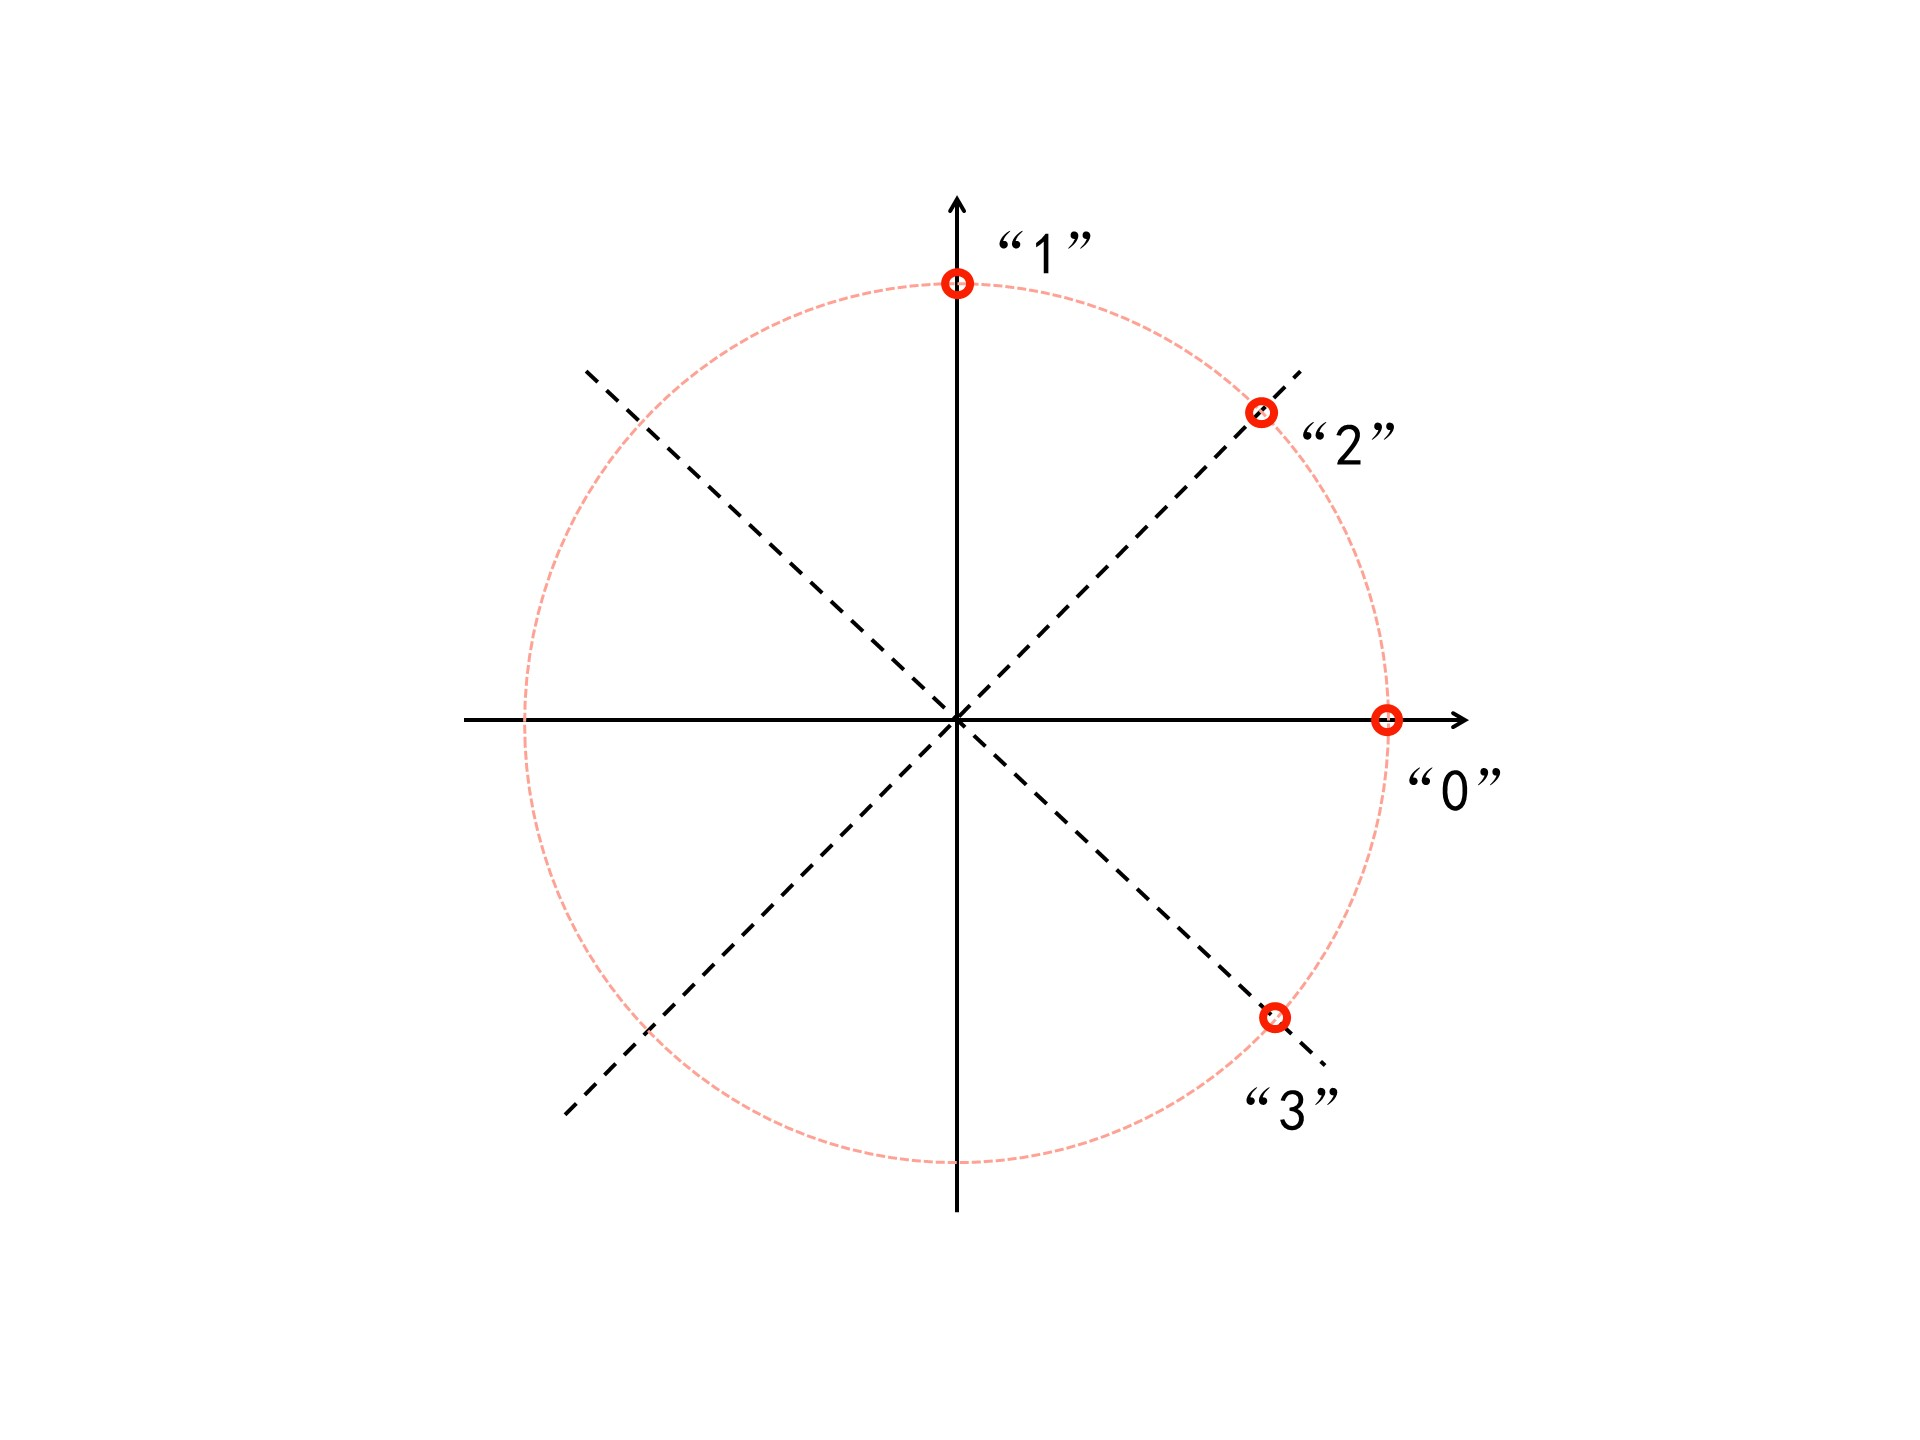
\includegraphics[width=6cm]{pic/qqpsk.jpg}
\caption{Constenlation diagram of quantum $\theta$ shift keying}
\label{qQPSK}
\end{figure}

The $\keta{+}$ wave is a superposition wave of the $\keta{0}$ and $\keta{1}$ waves and is best used as the input wave for parallel processing.
\begin{figure}[ht]
\begin{quantikz}
    \lstick{\ket{0}} & \gate{H} & \qw \rstick{\ket{+}}
\end{quantikz}
\caption{Use H gate to produce $\keta{+}$ wave.}
\label{H+}
\end{figure}

The $\keta{-}$ wave is also a superposition wave of the $\keta{0}$ and $\keta{1}$ waves, but is mostly used as the input wave phase kickback algorithm, which will be described in the following chapter.
\begin{figure}[ht]
\begin{quantikz}
    \lstick{\ket{0}} & \gate{X} & \gate{H} & \qw \rstick{\ket{-}}
\end{quantikz}
\caption{Use H gate to produce $\keta{-}$ wave.}
\label{H-}
\end{figure}

\section{Quantum gates for information processing}
Qubits are memory devices or communication channels. Quantum gates are processing devices that can change the modulation of $\theta$ and phase $\varphi$. As desired by the algorithms, the gates are concatenated or connected into circuits. Amplitude or the number of qubits is never changed until demodulation when qubits are measured. Measurements absorb the energy of qubits to extract digital data from them.

In the ket notation developed by physicists, a qubit gate operation is a quantum operator and can be noted by a letter $G$. In vector notation, a gate process can always be represented by a matrix. For example,
\begin{equation}
    \begin{pmatrix}
    cos\theta & e^{i\varphi} sin\theta \\
    e^{-i\varphi} sin\theta & cos\theta
    \end{pmatrix}
\end{equation}
which is unitary.
A algorithm or protocol is always depicted by a circuit diagram or series of matrix calculations. In circuit diagram, a qubit is shown as a line, and a gate as a rectangle.

\section{Hadamard gate}
Hadamard gate rotates the polarization $\theta$ of a qubit by 45 degrees. Its circuit symbol is letter "H" enclosed in a square. Rotating a $\keta{0}$ qubit 45 degrees obvious becomes a qubit of 45 degree polarization.
\begin{figure}[ht]
\begin{quantikz}
    \qw & \gate{H} &\qw
\end{quantikz}
\caption{Hadamard gate}
\label{Hadamard}
\end{figure}

\section{Pauli X, Y and Z gates}
A Z rotates a qubit's phase $\varphi$ by $180^{\circ}$ or $\pi$. A X gate exchanges $\keta{0}$ and $\keta{1}$. A Y gate exchanges $\keta{0}$ and $\keta{1}$ with additional phase change. They are best expressed in the vector notation as the Pauli matrices:
\begin{equation}
\begin{array}{rl}
    \sigma_1 & = \sigma_x = \begin{pmatrix}
        0 & 1 \\
        1 & 0
    \end{pmatrix} \\
    \sigma_2 & = \sigma_y = \begin{pmatrix}
        0 & -i \\
        i & 0
    \end{pmatrix} \\
    \sigma_3 & = \sigma_z = \begin{pmatrix}
        1 & 0 \\
        0 & -1
    \end{pmatrix}
\end{array}
\end{equation}
